\section{Results}
\label{sec:results}

We find one event in the signal region D. The event is in the $e\mu$ channel and contains 3 jets.
The SM MC expectation is 1.3 events.

Table~\ref{tab:datayield} summarizes the event yields obtained for each of the four ABCD 
regions in the data and in the  MC samples.
The prediction of the ABCD method is given by 
$N_\textrm{A}\times{}N_\textrm{C}/N_\textrm{B} = 1.3 \pm 0.8~(\textrm{stat.}) \pm 0.3~(\textrm{syst.})$ events.
The data, together with SM expectations, are presented in Figure~\ref{fig:abcdData}.

\begin{figure}[tbh]
\begin{center}
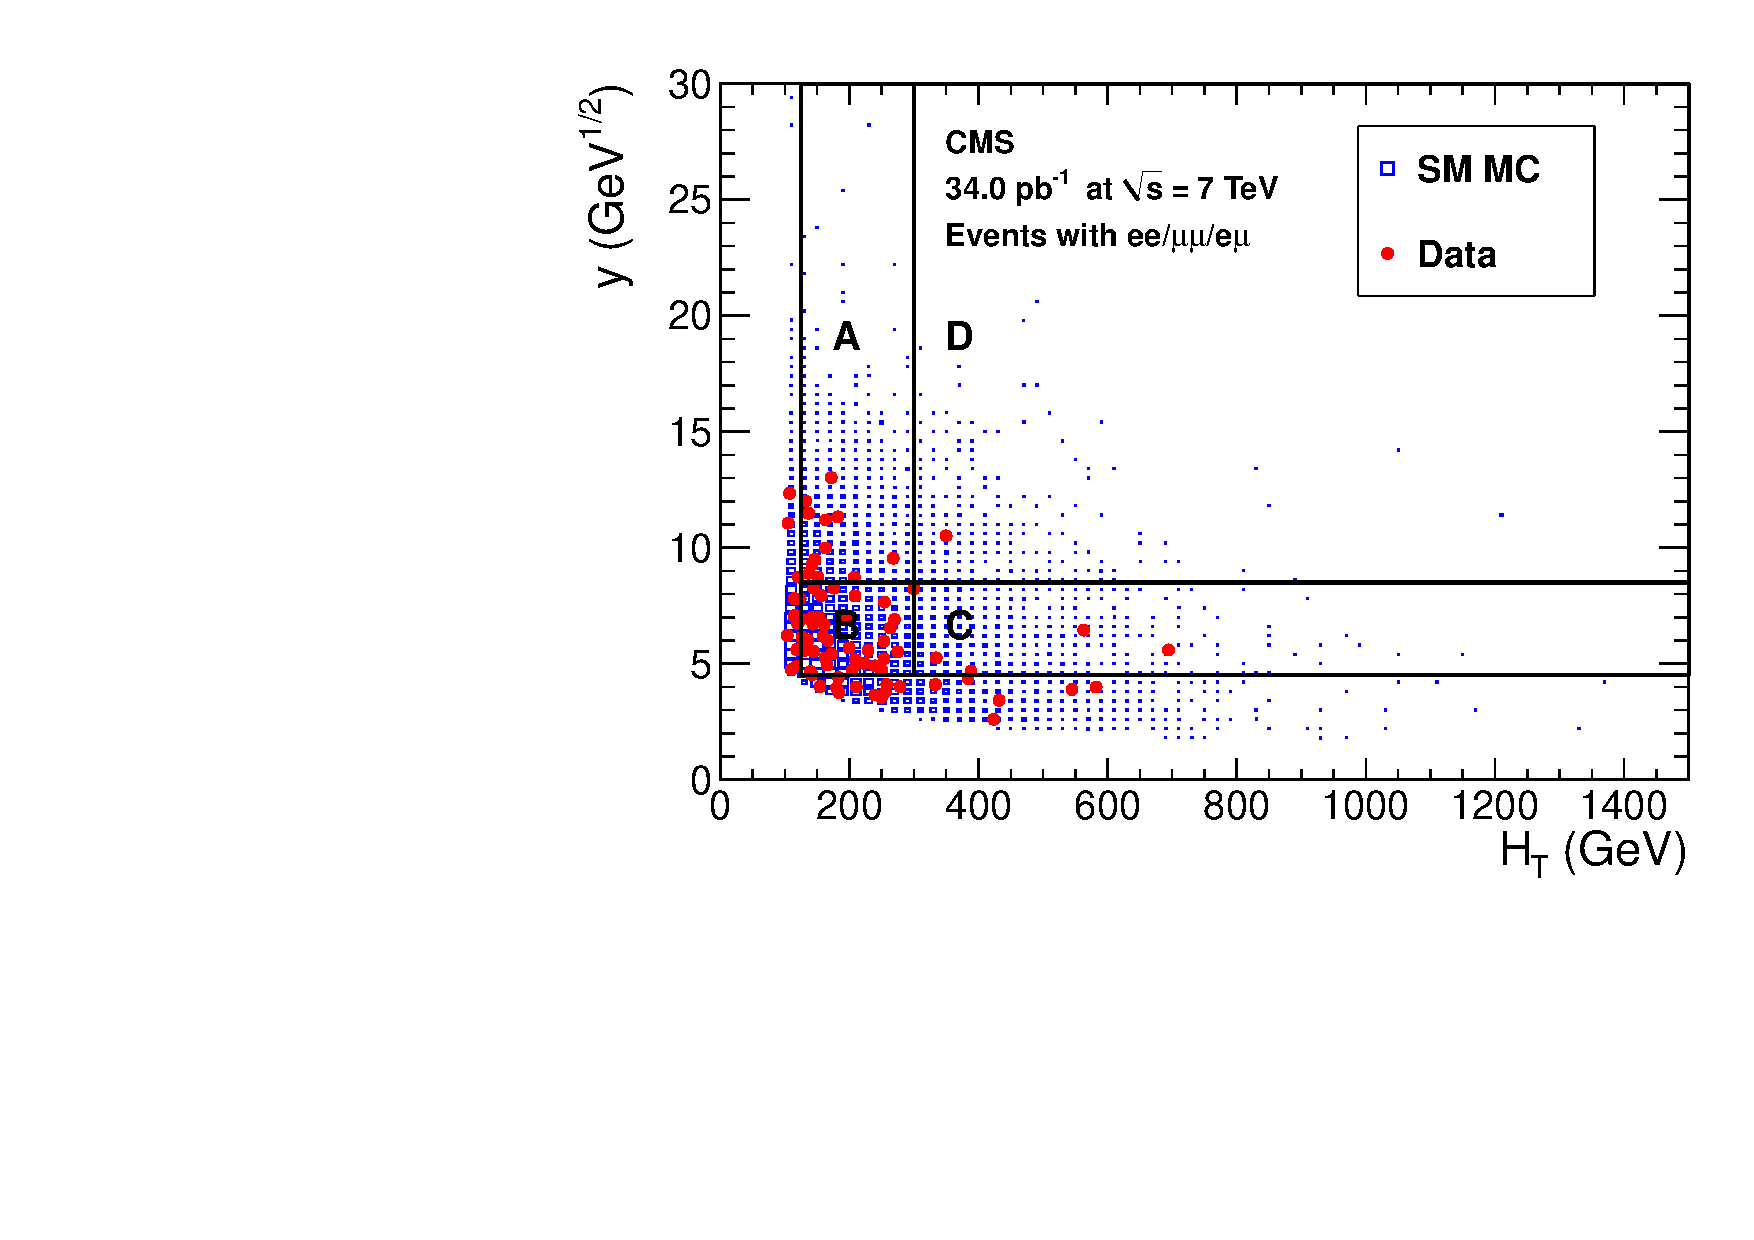
\includegraphics[width=0.75\linewidth]{plots_final/abcd.pdf}
\caption{\label{fig:abcdData}\protect Distributions of $y$ vs.\ \HT\   
for SM MC (2-dimensional histogram) and data (scatter plot).  Here  our 
choice of the ABCD regions is also shown.}
\end{center}
\end{figure}


\begin{table}[hbt]
\begin{center}
\caption{\label{tab:datayield} Data yields in the four
regions of Figure~\ref{fig:abcdData}, as well as the predicted yield in region D given
by $N_\textrm{A}\times{}N_\textrm{C}/N_\textrm{B}$. The SM and BSM MC expectations are also shown.  
The quoted uncertainties are statistical only.}
\vspace{2 mm}
\begin{tabular}{l||c|c|c|c||c}
\hline
              Sample                    &        $N_\text{A}$  &         $N_\text{B}$  &         $N_\text{C}$  &          $N_\text{D}$ &$N_\textrm{A}\times{}N_\textrm{C}/N_\textrm{B}$\\
\hline
$t\bar{t}\rightarrow \ell^{+}\ell^{-}$  &  8.44  $\pm$  0.18   &  32.83  $\pm$  0.35   &   4.78  $\pm$  0.14   &   1.07  $\pm$  0.06   &   1.23  $\pm$  0.05  \\
$t\bar{t}\rightarrow \mathrm{other}$    &  0.12  $\pm$  0.02   &   0.78  $\pm$  0.05   &   0.16  $\pm$  0.02   &   0.02  $\pm$  0.01   &   0.02  $\pm$  0.01  \\
Drell--Yan                               &  0.17  $\pm$  0.08   &   1.18  $\pm$  0.22   &   0.04  $\pm$  0.04   &   0.12  $\pm$  0.07   &   0.01  $\pm$  0.01  \\
    $W^{\pm}$ + jets                    &  0.00  $\pm$  0.00   &   0.09  $\pm$  0.09   &   0.00  $\pm$  0.00   &   0.00  $\pm$  0.00   &   0.00  $\pm$  0.00  \\
            $W^+W^-$                    &  0.11  $\pm$  0.01   &   0.29  $\pm$  0.02   &   0.02  $\pm$  0.01   &   0.03  $\pm$  0.01   &   0.01  $\pm$  0.00  \\
        $W^{\pm}Z$                      &  0.01  $\pm$  0.00   &   0.04  $\pm$  0.00   &   0.00  $\pm$  0.00   &   0.00  $\pm$  0.00   &   0.00  $\pm$  0.00  \\
            $ZZ$                        &  0.01  $\pm$  0.00   &   0.02  $\pm$  0.00   &   0.00  $\pm$  0.00   &   0.00  $\pm$  0.00   &   0.00  $\pm$  0.00  \\
          Single top                    &  0.29  $\pm$  0.01   &   1.04  $\pm$  0.03   &   0.04  $\pm$  0.01   &   0.01  $\pm$  0.00   &   0.01  $\pm$  0.00  \\
\hline
         Total SM MC                    &  9.14  $\pm$  0.20   &  36.26  $\pm$  0.43   &   5.05  $\pm$  0.14   &   1.27  $\pm$  0.10   &   1.27  $\pm$  0.05  \\
\hline
                Data                    &                 12   &                  37   &                   4   &                   1   &   1.30  $\pm$  0.78  \\
\hline
\hline
                 LM0                    &   4.04  $\pm$  0.19  &   4.45  $\pm$  0.20   &  13.92  $\pm$  0.36   &   8.63  $\pm$  0.27   &  12.63  $\pm$  0.88  \\
                 LM1                    &   0.52  $\pm$  0.02  &   0.26  $\pm$  0.02   &   1.64  $\pm$  0.04   &   3.56  $\pm$  0.06   &   3.33  $\pm$  0.27  \\
\hline
\end{tabular}
\end{center}
\end{table}



%%\subsection{Background estimate from the $\pt(\ell\ell)$ method}
%%\label{sec:victoryres}

The ABCD prediction is then compared with that of the $\pt(\ell \ell)$ method.
We find 1 event passing the requirements $\HT > 300\GeV$ and 
$\pt(\ell\ell)/\sqrt{\HT} > 8.5\GeV^{1/2}$. This leads to a predicted
background of $2.1 \pm 2.1~({\rm stat.}) \pm 0.6~({\rm syst.})$ after applying
the correction factor $K_{50} \times K_C = 2.1 \pm 0.6$,
as shown in Figure~\ref{fig:victory} (left).

As a validation of the $\pt(\ell\ell)$ method in a region with higher statistics,
we also apply the $\pt(\ell\ell)$ method in control region A by restricting
\HT\ to be in the range 125--300~\GeV. Here the prediction is $9.0 \pm 6.0~(\textrm{stat.})$
background events, in good agreement with the observed yield of 12 events, as shown
in Figure~\ref{fig:victory} (right).

\begin{figure}[hbt]
\begin{center}
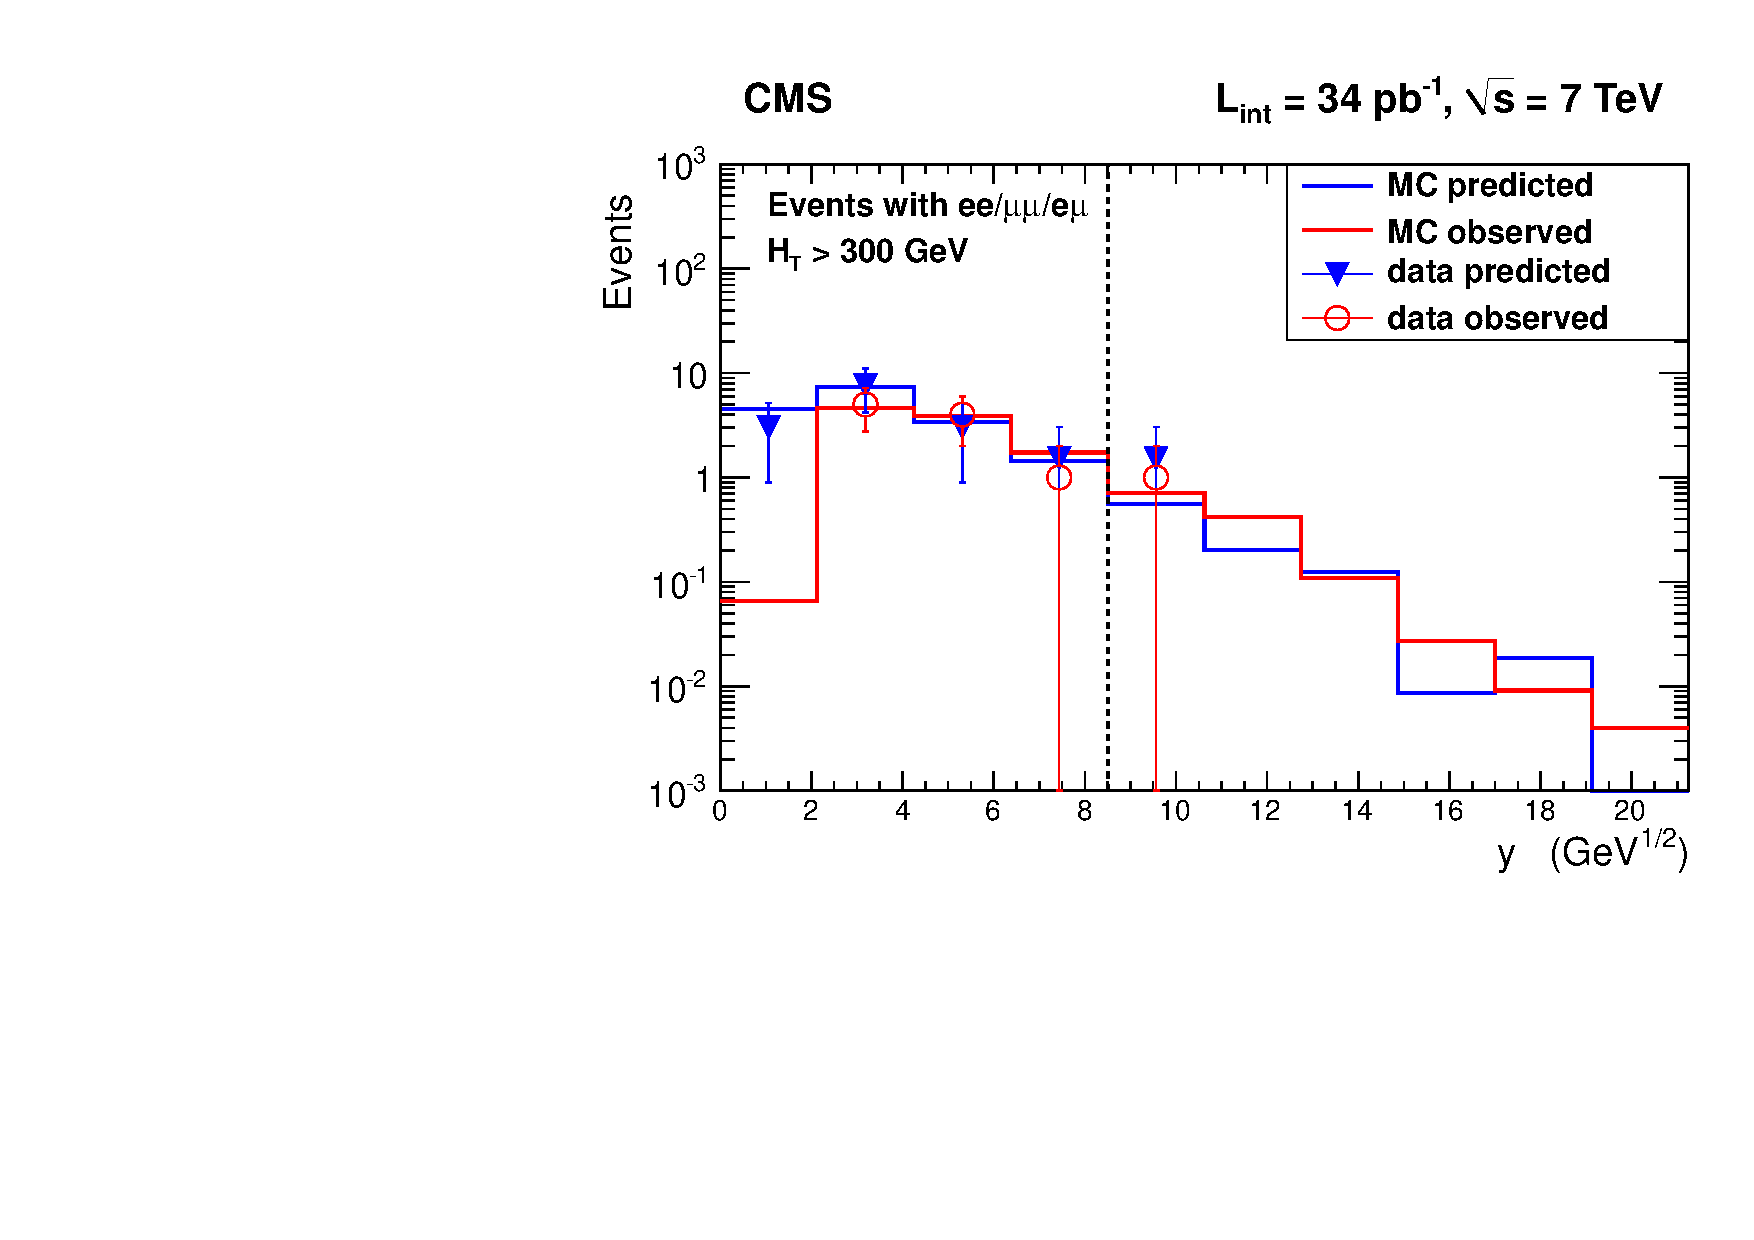
\includegraphics[width=0.49\linewidth]{plots_final/victory_signal.pdf}
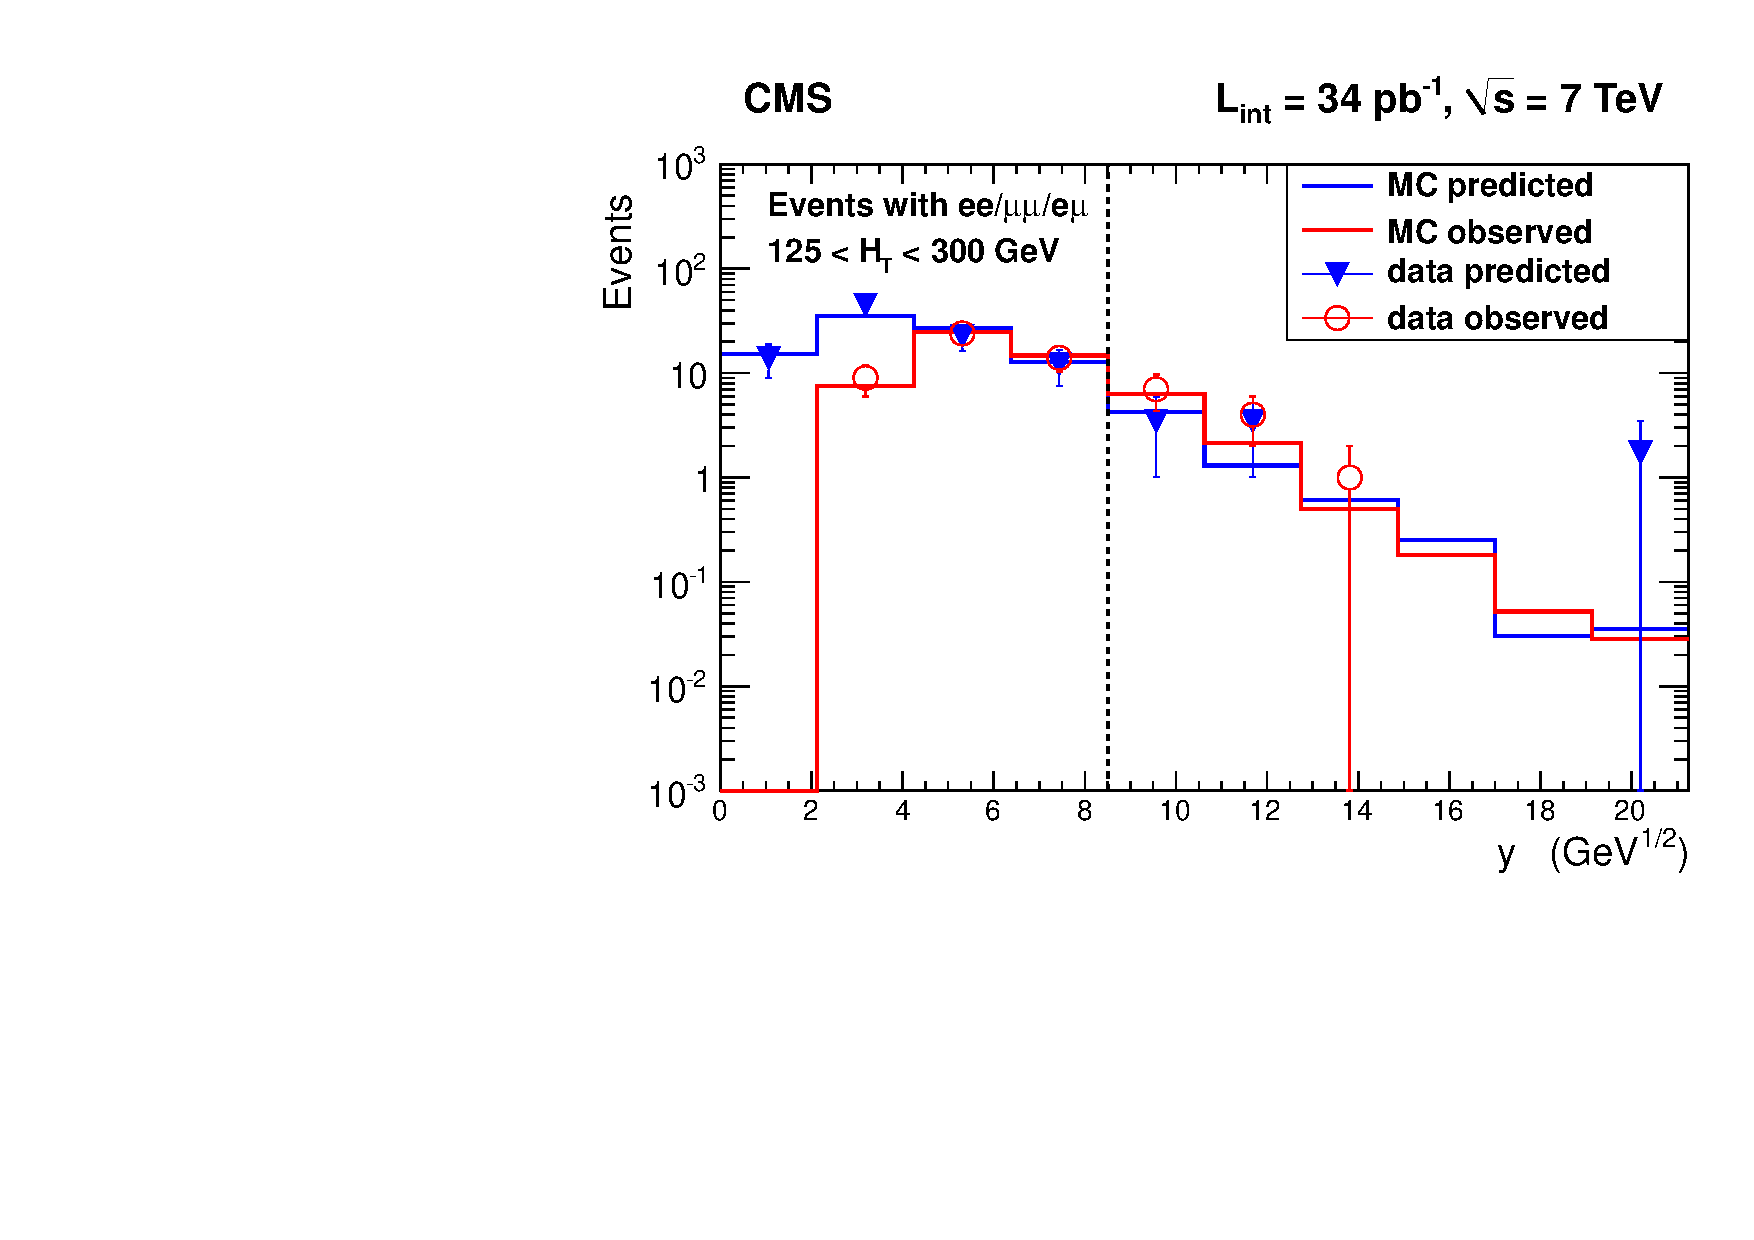
\includegraphics[width=0.49\linewidth]{plots_final/victory_control.pdf}
\caption{\label{fig:victory}\protect Distributions of 
$y$ (observed) and ${\pt(\ell\ell)}/\sqrt{\HT}$ scaled by the correction
factor $K_{50}$ (predicted)
for (left) the signal region and (right) the control region A, for both MC and data.
The vertical dashed line indicates the search region defined by $y>8.5\GeV^{1/2}$.
The deficit at low $y$ is due to the $\MET > 50\GeV$ preselection requirement.}
\end{center}
\end{figure}



%\begin{table}[hbt]
%\begin{center}
%\caption{\label{tab:victory} The predictions of the $\pt(\ell \ell)$ method and observed event yields in the signal region 
%and control region A. The predicted yield for data has been scaled by $K_C$, which is the ratio of observed to predicted
%yields in MC. The uncertainties are statistical only. }
%\vspace{2 mm}
%\begin{tabular}{l|cc|cc}
%\hline
%              &   Signal Region    &              &  Control Region     &                         \\
%\hline                                                                                                    
%              &   Predicted        &  Observed    &  Predicted          &   Observed              \\              
%\hline                                                                                                    
%total SM   MC &   0.9              &  1.3         &       6.5           &        9.1              \\
%         data &   $2.1 \pm 2.1$    &  1           &  $9.0 \pm 6.0$      &         12              \\
%\hline
%\end{tabular}
%\end{center}
%\end{table}

%\begin{table}[hbt]
%\begin{center}
%\caption{\label{tab:victory_signal}Results of the dilepton \pt\ template method in the signal region
%$\mathrm{sumJetPt} > 300\GeV$. The predicted and observed yields for
%the region $\mathrm{tcmet}/\sqrt{\mathrm{sumJetPt}}>$~8.5 are shown for data
%and MC. The error on the prediction for data is statistical only, assuming
%Gaussian errors.}
%\begin{tabular}{lccc}
%\hline
%              & Predicted                &   Observed &  Obs/Pred \\
%\hline
%total SM   MC &      1.03                &       1.43 &      1.38 \\
%         data &    $2.53 \pm 2.25$       &          1 &      0.40 \\
%\hline
%\end{tabular}
%\end{center}
%\end{table}%

%\clearpage

In summary, for the signal region defined as $\HT>300\GeV$ and $y > 8.5\GeV^{1/2}$: 
we observe one event in the data, 
SM MC predicts 1.3 events, 
the ABCD method predicts $1.3 \pm 0.8~({\rm stat.}) \pm 0.3~({\rm syst.})$ events, 
and the $\pt(\ell\ell)$ method predicts $2.1 \pm 2.1~({\rm stat.}) \pm 0.6~({\rm syst.})$ events.

All three background predictions are consistent within their uncertainties.
We thus take as our best estimate of the SM yield in 
the signal region the error-weighted average of the two background estimates based on data and find 
a number of predicted background events $N_\textrm{BG}=1.4 \pm 0.8$, in good agreement with the 
observed signal yield. We therefore conclude that no evidence for a non-SM contribution 
to the signal region is observed.







